\subsection{Practice 7}

\begin{enumerate}
    \item Find the volume of a cone with radius $r$ and height $h$ using definite
          integrals. \sol{}

          Let $y$ be the height of any cross section of the cone, and $x$ be the radius
          of the cross section.
          \begin{flalign*}
              \dfrac{y}{h} & = \dfrac{x}{r}   & \\
              y            & = \dfrac{h}{r} x
          \end{flalign*}
          \begin{flalign*}
              V & = \int_0^h \pi y^2 d x                                  & \\
                & = \int_0^h \pi \left(\dfrac{h}{r} x\right)^2 d x        & \\
                & = \pi \dfrac{h^2}{r^2} \int_0^h x^2 d x                 & \\
                & = \pi \dfrac{h^2}{r^2} \left[\dfrac{1}{3}x^3\right]_0^h & \\
                & = \pi \dfrac{h^2}{r^2} \cdot \dfrac{1}{3}h^3            & \\
                & = \dfrac{1}{3} \pi r^2 h
          \end{flalign*}

    \item Shown in the diagram below is the shaded region bounded by the ellipse
          $\dfrac{x^2}{a^2} + \dfrac{y^2}{b^2} = 1$, where $a > 0$ and $b > 0$. If the
          volume of the solid of revolution formed by rotating this region about the
          $x$-axis and the $y$-axis is $V_x$ and $V_y$ respectively,
          \begin{center}
              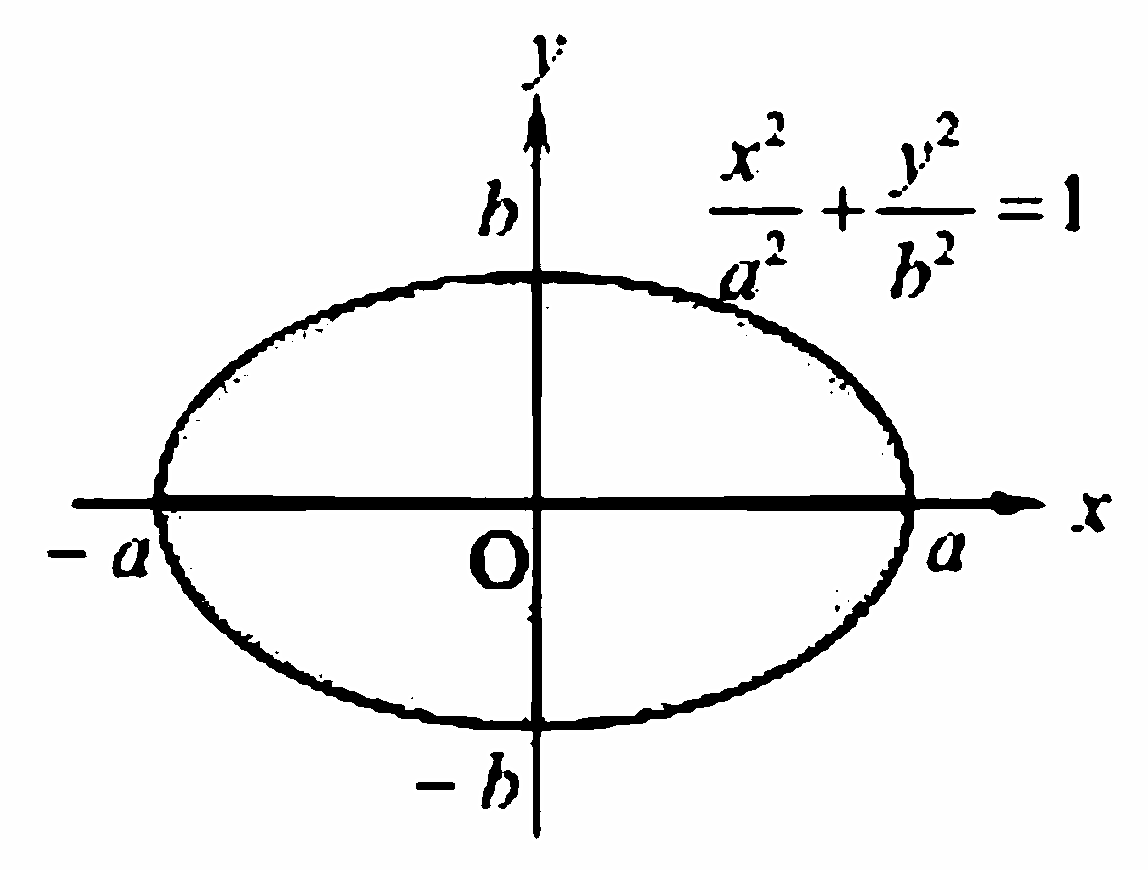
\includegraphics[width=0.3\textwidth]{assets/28-prac7-2.png}
          \end{center}
          \begin{enumerate}
              \item find $V_x$ and $V_y$. \sol{} \vspace{-0.8cm}
                    \begin{multicols}{2}
                        \begin{flalign*}
                            \dfrac{x^2}{a^2} + \dfrac{y^2}{b^2} & = 1                                    & \\
                            \dfrac{y^2}{b^2}                    & = 1 - \dfrac{x^2}{a^2}                 & \\
                            y^2                                 & = b^2\left(1 - \dfrac{x^2}{a^2}\right)
                        \end{flalign*}
                        \begin{flalign*}
                            V_x & = \int_{-a}^a \pi y^2 d x                                                  & \\
                                & = \pi b^2 \int_{-a}^a \left(1 - \dfrac{x^2}{a^2}\right) d x                & \\
                                & = \pi b^2 \left[x - \dfrac{x^3}{3a^2}\right]_{-a}^a                        & \\
                                & = \pi b^2 \left[a - \dfrac{a^3}{3a^2} - (-a) + \dfrac{(-a)^3}{3a^2}\right] & \\
                                & = \pi b^2 \left[a - \dfrac{a}{3} + a - \dfrac{a}{3}\right]                 & \\
                                & = \dfrac{4}{3} \pi a b^2
                        \end{flalign*}
                        \vfill\null\columnbreak
                        \begin{flalign*}
                            \dfrac{x^2}{a^2} + \dfrac{y^2}{b^2} & = 1                                    & \\
                            \dfrac{x^2}{a^2}                    & = 1 - \dfrac{y^2}{b^2}                 & \\
                            x^2                                 & = a^2\left(1 - \dfrac{y^2}{b^2}\right)
                        \end{flalign*}
                        \begin{flalign*}
                            V_y & = \int_{-b}^b \pi x^2 d y                                                           & \\
                                & = \pi a^2 \int_{-b}^b \left(1 - \dfrac{y^2}{b^2}\right) d y                         & \\
                                & = \pi a^2 \left[y - \dfrac{y^3}{3b^2}\right]_{-b}^b                                 & \\
                                & = \pi a^2 \left[b - \dfrac{b^3}{3b^2} - (-b) + \dfrac{(-b)^3}{3b^2}\right]          & \\
                                & = \pi a^2 \left[b - \dfrac{b}{3} + b - \dfrac{b}{3}\right] = \dfrac{4}{3} \pi a^2 b
                        \end{flalign*}
                    \end{multicols}
                    \vspace{-1cm}

              \item if $V_x = 3V_y$, find the value of $a:b$. \sol{}
                    \begin{flalign*}
                        \dfrac{4}{3} \pi a b^2 & = 3 \cdot \dfrac{4}{3} \pi a^2 b & \\
                        4\pi a b^2             & = 12 \pi a^2 b                   & \\
                        b                      & = 3a                             & \\
                        a:b                    & = 1:3
                    \end{flalign*}
          \end{enumerate}
\end{enumerate}